
\section{\trFloerEquation{}的\trLinearization：\texorpdfstring{$\scr{F}$}{F} 的\trDifferential{}的计算}
\label{sec:linearization-floer}

为了使初学者免受\trVectorField{}求导之苦以及\trLeviCivita（Levi-Cività）\trConnection{}的使用之苦，我们将利用 $W$ 在 $\RR^m$ 中的一个\trEmbedding（$m$ 非常大，无论如何都大于该\trManifold{}的维数 $2n$）。令
\[
TW\subset\RR^m\times\RR^m\xrightarrow{\ \mathrm{pr}_2\ }\RR^m\text{，}
\]
诸向量 $Z_i$，以及所有沿 $u$ 切于 $W$ 的向量、甚至沿 $u$ 的一个邻域 $B$ 切于 $W$ 的向量，都可以被看成 $\RR^m$ 中的向量。同样地，我们把 $\scr{F}$ 看成在一个由取值于 $\RR^m$ 的映射组成的\trVectorSpace{}中取值，也就是 $\cC^\infty(\RR\times S^1;\RR^m)$ 或 $L^p(\RR\times S^1;\RR^m)$。为了计算 $\scr{F}$ 的\trDifferential，我们于是取定\trFloerEquation{}的一个解
\[
u\in\scr{M}(x,y)\subset\cC^\infty_{\mathrm{loc}}(\RR\times S^1;W)
\]
圆柱
\[
u\colon\RR\times S^1\longrightarrow W
\]
可以补全成一张\trSphere：\trLoop{} $x$ 与 $y$ 都是\trContractible{}的，我们把它们扩张成两个\trDisk，这就得到一个映射
\[
\widetilde{u}\colon S^2\longrightarrow W
\]
如\cref{fig:capped-cylinder}所示。

\begin{figure}[htbp]
\centering
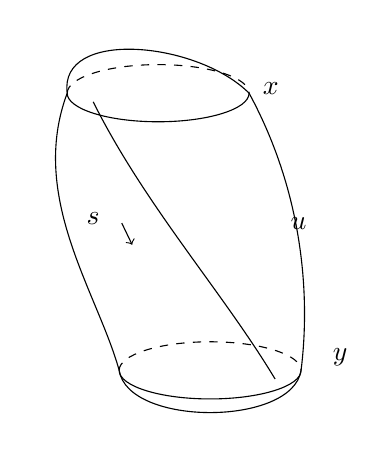
\begin{tikzpicture}[scale=1.1]
\draw (-1.05,0) .. controls (-1.15,0.75) and (0.45,0.6) .. (1.05,0);
\draw[dashed] (-1.05,0) arc (180:0:1.05 and 0.33);
\draw (-1.05,0) arc (180:360:1.05 and 0.33);
\draw[dashed] (-0.45,-3.2) arc (180:0:1.05 and 0.33);
\draw (-0.45,-3.2) arc (180:360:1.05 and 0.33);
\draw (-0.45,-3.2) .. controls (-0.35,-3.85) and (1.55,-3.85) .. (1.65,-3.2);
\draw (-1.05,0) .. controls (-1.5,-1.2) and (-0.7,-2.3) .. (-0.45,-3.2);
\draw (1.05,0) .. controls (1.7,-1.2) and (1.75,-2.4) .. (1.65,-3.2);
\draw (-0.75,-0.1) .. controls (-0.15,-1.3) and (0.75,-2.3) .. (1.35,-3.3);
\draw[->] (-0.42,-1.5) -- (-0.3,-1.75);
\node at (1.3,0.05) {$x$};
\node at (2.1,-3.05) {$y$};
\node at (1.62,-1.5) {$u$};
\node at (-0.75,-1.45) {$s$};
\end{tikzpicture}
\caption{}
\label{fig:capped-cylinder}
\end{figure}

如第 7 章中那样，\trFiberBundle{} $\widetilde{u}^\star TW$ 可以作为一个\trSymplectic{}\trFiberBundle{}被\trTrivialization（得益于\cref{thm:symplectic-trivialization}）。于是我们选取一个\trTrivialization，也就是一个属于 $T_{u(s,t)}W$ 的基 $(Z_1,\dots,Z_{2n})$，它以 $\cC^\infty$ 方式依赖于 $s$ 与 $t$（此处我们把诸 $(s,t)$ 的圆柱 $\RR\times S^1$ 视为该\trSphere{}的一个子集，如\cref{fig:capped-cylinder}所示）。我们将要求这个\trTrivialization{}是\trSymplectic{}且\trOrthonormal{}的，也就是说，由诸 $Z_i$ 组成的基是一个\trSymplectic{}且\trOrthonormal{}的基，并且诸向量 $Z_i$ 在 $s$ 趋于 $\pm\infty$ 时有极限。我们还需要
\[
\lim_{s\to\pm\infty}\frac{\partial Z_i}{\partial s}=0,
\qquad
\lim_{s\to\pm\infty}\frac{\partial^2 Z_i}{\partial s^2}=0,
\qquad
\lim_{s\to\pm\infty}\frac{\partial^2 Z_i}{\partial s\,\partial t}=0\text{。}
\]
这样一些\trTrivialization{}确实存在，我们可以借助于\cref{fig:capped-cylinder}中球冠附近的圆柱使自己确信这一点。

这个\trFrame{}定义了\trBanachManifold{} $\scr{P}^{1,p}(x,y)$ 的一个（以 $u$ 为中心的）\trChart：
\[
\begin{array}{c}
i\colon W^{1,p}(\RR\times S^1;\RR^{2n})\longrightarrow\scr{P}^{1,p}(x,y)\\[4pt]
(y_1,\dots,y_{2n})\longmapsto\exp_u\Bigl(\sum y_iZ_i\Bigr)\text{。}
\end{array}
\]
注意到
\[
(di)_0(y_1,\dots,y_{2n})=\sum y_iZ_i
\]
（因为 $(d\exp)_0=\mathrm{Id}$；必要时参见\cref{sec:riemannian-metrics-exp}）。

现在让我们考虑下面这个映射，我们仍把它称作 $\scr{F}$：
\[
\begin{array}{c}
\scr{F}\colon\scr{P}^{1,p}(x,y)\xrightarrow{\ \scr{F}\ }L^p(\RR\times S^1;TW)\longrightarrow L^p(\RR\times S^1;\RR^m)\\[6pt]
u\longmapsto\dfrac{\partial u}{\partial s}+J(u)\Bigl(\dfrac{\partial u}{\partial t}-X_t(u)\Bigr)
\end{array}
\]
并让我们计算它在 $u$ 处的\trDifferential。令
\[
Y(s,t)=\bigl(y_1(s,t),\dots,y_{2n}(s,t)\bigr)\in\RR^{2n}\subset\RR^m
\]
为一个向量。我们把 $Y=\sum y_iZ_i$ 视为 $\RR^m$ 中切于 $W$ 的一个向量。让我们写
\[
\scr{F}(u+Y)=\frac{\partial(u+Y)}{\partial s}+J(u+Y)\frac{\partial(u+Y)}{\partial t}-J(u+Y)X_t(u+Y)\text{。}
\]
这个表达式中关于 $Y$ 为线性的部分是
\[
(d\scr{F})_u(Y)=\frac{\partial Y}{\partial s}+(dJ)_u(Y)\frac{\partial u}{\partial t}+J(u)\frac{\partial Y}{\partial t}-(dJ)_u(Y)X_t-J(u)(dX_t)_u(Y)\text{。}
\]

\begin{lemma}\label{thm:df-product-rule}
对于每个在 $\RR^m$ 的\trEndomorphism{}中取值的映射 $J$，以及所有在 $\RR^m$ 中取值的映射 $Y$ 与 $v$，我们有
\[
(dJ)(Y)\cdot v=d(Jv)(Y)-J\,dv(Y)\text{。}
\]
\end{lemma}

\begin{proof}
只需对映射 $x\mapsto J(x)\cdot v(x)$ 求导，这就给出
\[
J(x+Y)\cdot v(x+Y)=\bigl(J(x)+(dJ)_x(Y)\bigr)\cdot\bigl(v(x)+(dv)_x(Y)\bigr)
\]
（精确到一阶），于是
\[
d(J\cdot v)_x(Y)=(dJ)_x(Y)\cdot v(x)+J(x)\cdot(dv)_x(Y)\text{。}
\]
\end{proof}

\begin{remark}\label{thm:df-order-decomposition}
对每个 $\cC^\infty$ 类的映射 $u\colon\RR\times S^1\to W$，
\[
(d\scr{F})_u(Y)=\Bigl(\frac{\partial Y}{\partial s}+J(u)\frac{\partial Y}{\partial t}\Bigr)+\Bigl((dJ)_u(Y)\frac{\partial u}{\partial t}-(dJ)_u(Y)X_t-J(u)(dX_t)_u(Y)\Bigr)
\]
是一个一阶\trDifferential{}算子与一个零阶算子之和。现在让我们使用由基 $(Z_1,\dots,Z_{2n})$ 定义的\trChart，并写
\[
Y=\sum y_iZ_i\text{。}
\]
在这个\trChart{}中，我们有
\[
\begin{aligned}
(d\scr{F})_u(Y)&=\sum\Bigl(\frac{\partial y_i}{\partial s}Z_i+\frac{\partial y_i}{\partial t}J(u)Z_i\Bigr)\\
&\qquad+\sum y_i\Bigl(\frac{\partial Z_i}{\partial s}+J(u)\frac{\partial Z_i}{\partial t}+(dJ)_u(Z_i)\frac{\partial u}{\partial t}\\
&\qquad\qquad-J(u)(dX_t)_uZ_i-(dJ)_u(Z_i)X_t\Bigr)\text{。}
\end{aligned}
\]
第一行的那些项是“一阶的”，也就是说它们对 $y_i$ 求导\footnote{译注：原书此处称第一行诸项为“零阶的”（“that is, they do not differentiate the $y_i$”，即不对 $y_i$ 求导），而称先研究“一阶”项、“即余下的那些项”——与上式两行的实际阶数（首行含 $\partial y_i/\partial s$ 与 $\partial y_i/\partial t$，余下各项仅以 $y_i$ 线性出现、不含其导数）以及本注记后文的分类（一阶项即 $\bar{\partial}(y_1,\dots,y_{2n})$）恰相反，疑系排印颠倒，此处径改。——译者注}。我们先来研究这些“一阶”项。容易看出它们可化为
\[
\sum\Bigl(\frac{\partial y_i}{\partial s}+J_0\frac{\partial y_i}{\partial t}\Bigr)Z_i\text{，}
\]
其中 $J_0$ 是 $\RR^{2n}=\CC^n$ 上的标准\trComplexStructure。

我们也可以说，\trLinearization{}后的\trFloerEquation{}是\trCauchyRiemann{}算子与一个零阶算子之和。的确，我们有：
\begin{itemize}
\item 既然已假设基 $Z_1,\dots,Z_{2n}$ 是\trSymplectic{}且\trOrthonormal{}的，那么一阶项就是 $\bar{\partial}(y_1,\dots,y_{2n})$，其中 $\bar{\partial}$ 表示标准\trComplexStructure\footnote{差一个因子 $2$：通常的 $\bar{\partial}$ 是 $\frac{1}{2}\Bigl(\dfrac{\partial}{\partial s}+J_0\dfrac{\partial}{\partial t}\Bigr)$。} $J_0$ 的\trCauchyRiemann{}算子。
\item 另外两项不对 $y_i$ 求导（这的确是一个零阶算子）。
\end{itemize}
\end{remark}

\begin{remark}[关于记号]\label{thm:chart-notation}
一如既往，要写下一个定义在\trManifold{}上的映射的\trDifferential，我们需要这个\trManifold{}的一个\trChart。这里我们所用的是
\[
F_u\colon W^{1,p}(\RR\times S^1;\RR^{2n})\longrightarrow\scr{P}^{1,p}(x,y)\xrightarrow{\ \scr{F}\ }L^p(\RR\times S^1;\RR^m)\text{，}
\]
其中第一个映射就是那个以 $u$ 为中心的\trChart（即前文记作 $i$ 的那个映射）。当然，$(d\scr{F})_u$ 表示的就是在坐标之下为 $(dF_u)_0$ 的那个东西。我们不认为使用记号 $(dF_u)_0$ 会对本文的清晰性有所助益，因此我们没有使用它。
\end{remark}

\cref{thm:df-order-decomposition}中的等式表明，在这个\trChart{}中，$(d\scr{F})_u$ 可以分解成
\[
(d\scr{F})_u(Y)=\bar{\partial}Y+SY\text{，}
\]
其中 $S$ 是一个零阶\trLinearOperator，它可以被看成一个\trSmooth{}映射\footnote{译注：原书此处印作 $\operatorname{End}(\RR^{n})$；按 $S$ 作用于 $Y\in\RR^{2n}$（下文的同款映射（p.240）印 $\operatorname{End}(\RR^{2n})$），疑为漏印下标 $2$，此处径改。——译者注}
\[
S\colon\RR\times S^1\longrightarrow\operatorname{End}(\RR^{2n})\text{。}
\]

在 $u$ 是\trFloerEquation{}的一个解的情形，这个零阶算子具有一条特殊的性质。

\begin{proposition}\label{thm:df-dbar-plus-s}
若 $u$ 是\trFloerEquation{}的一个解，则 $\scr{F}$ 在 $u$ 处的\trDifferential{}是一个和
\[
(d\scr{F})_u=\bar{\partial}+S(s,t)\text{，}
\]
其中 $S$ 是一个\trLinearOperator，它在 $s$ 趋于 $\pm\infty$ 时趋于一个对称算子，并且满足
\[
\lim_{s\to\pm\infty}\frac{\partial S}{\partial s}(s,t)=0
\]
（关于 $t$ \trUniform）。
\end{proposition}

\begin{proof}[\cref{thm:df-dbar-plus-s}的证明]
我们从\cref{thm:df-order-decomposition}所给的表达式出发；算子 $S$ 就是其中的零阶部分：
\[
S(y_1,\dots,y_{2n})=\sum y_i\Bigl[\frac{\partial Z_i}{\partial s}+(dJ)_u(Z_i)\Bigl(\frac{\partial u}{\partial t}-X_t(u)\Bigr)+J(u)\frac{\partial Z_i}{\partial t}-J(u)(dX_t)_u(Z_i)\Bigr]\text{。}
\]
当 $s$ 趋于 $\pm\infty$ 时
\[
\lim\Bigl(\frac{\partial u}{\partial t}-X_t(u)\Bigr)=0
\]
因为 $u$ 是一个解，而 $\partial u/\partial s$（当 $s\to\pm\infty$ 时）\trUniform{}地趋于 $0$，其导数亦然（参见\cref{thm:trajectories-tend-critical-points}与\cref{thm:second-derivatives-vanish}）。其次，我们所选取的诸 $Z_i$ 满足
\[
\lim_{s\to\pm\infty}\frac{\partial Z_i}{\partial s}=0\text{，}
\]
它们的导数亦然。于是我们得到
\[
\lim_{s\to\pm\infty}\frac{\partial S}{\partial s}=0\text{。}
\]
由同样的论证，只需对 $s\to\pm\infty$ 证明算子
\[
A(y_1,\dots,y_{2n})=\sum y_i\Bigl(J(u)\frac{\partial Z_i}{\partial t}-J(u)(dX_t)_u(Z_i)\Bigr)
\]
的对称性。$A(y_1,\dots,y_{2n})$ 的第 $j$ 个分量是
\[
\sum y_i\Bigl\langle J(u)\frac{\partial Z_i}{\partial t}-J(u)(dX_t)_u(Z_i),Z_j\Bigr\rangle\text{；}
\]
于是让我们证明
\[
\lim_{s\to\pm\infty}\Bigl\langle J(u)\tfrac{\partial Z_i}{\partial t}-J(u)(dX_t)_u(Z_i),Z_j\Bigr\rangle-\Bigl\langle J(u)\tfrac{\partial Z_j}{\partial t}-J(u)(dX_t)_uZ_j,Z_i\Bigr\rangle=0\text{。}
\]
我们有（利用\trFrame{} $(Z_i)$ 是\trUnitary{}的这一事实）
\[
\begin{aligned}
0&=\frac{\partial}{\partial t}\bigl\langle J(u)Z_i,Z_j\bigr\rangle\\
&=\Bigl\langle(dJ)_u\Bigl(\frac{\partial u}{\partial t}\Bigr)Z_i,Z_j\Bigr\rangle+\Bigl\langle J(u)\frac{\partial Z_i}{\partial t},Z_j\Bigr\rangle+\Bigl\langle J(u)Z_i,\frac{\partial Z_j}{\partial t}\Bigr\rangle\\
&=\Bigl\langle(dJ)_u\Bigl(\frac{\partial u}{\partial t}\Bigr)Z_i,Z_j\Bigr\rangle+\Bigl\langle J(u)\frac{\partial Z_i}{\partial t},Z_j\Bigr\rangle-\Bigl\langle Z_i,J(u)\frac{\partial Z_j}{\partial t}\Bigr\rangle\text{。}
\end{aligned}
\]
因此，只需证明
\[
\lim_{s\to\pm\infty}\Bigl(\begin{aligned}[t]
&-\bigl\langle J(u)(dX_t)_u(Z_i),Z_j\bigr\rangle+\bigl\langle J(u)(dX_t)_u(Z_j),Z_i\bigr\rangle\\
&\qquad-\Bigl\langle(dJ)_u\Bigl(\frac{\partial u}{\partial t}\Bigr)Z_i,Z_j\Bigr\rangle
\end{aligned}\Bigr)=0\text{。}
\]
再一次利用
\[
\lim_{s\to\pm\infty}\Bigl(\frac{\partial u}{\partial t}-X_t(u)\Bigr)=0
\]
这一事实，这就等价于
\[
\lim_{s\to\pm\infty}\Bigl(\begin{aligned}[t]
&-\bigl\langle J(u)(dX_t)_u(Z_i),Z_j\bigr\rangle+\bigl\langle J(u)(dX_t)_u(Z_j),Z_i\bigr\rangle\\
&\qquad-\bigl\langle(dJ)_u(X_t)Z_i,Z_j\bigr\rangle
\end{aligned}\Bigr)=0\text{。}
\]
注意到，对一个取定的 $(s,t)$，这个表达式只依赖于诸 $Z_i$ 在点 $u(s,t)$ 处的取值。我们来证明下面这条引理。

\begin{lemma}\label{thm:symmetry-relation}
设 $p\in W$，并设 $(Z_i)_{i=1,\dots,2n}$ 是 $T_pW$ 的一个\trUnitary{}基。那么：
\[
-\bigl\langle J(p)(dX_t)_p(Z_i),Z_j\bigr\rangle+\bigl\langle J(p)(dX_t)_p(Z_j),Z_i\bigr\rangle-\bigl\langle(dJ)_p(X_t)Z_i,Z_j\bigr\rangle=0\text{。}
\]
\end{lemma}

\begin{proof}[\cref{thm:symmetry-relation}的证明]
把 $(Z_i)_{i=1,\dots,2n}$ 扩充成 $TW$ 在包含 $p$ 的一个\trChart{}定义域上的一个\trUnitary{}\trFrame。利用\cref{thm:df-product-rule}，上式就写成
\[
\begin{aligned}
&-\bigl\langle J(dX_t)(Z_i),Z_j\bigr\rangle+\bigl\langle J(dX_t)(Z_j),Z_i\bigr\rangle+\bigl\langle J(dZ_i)(X_t),Z_j\bigr\rangle-\bigl\langle d(JZ_i)(X_t),Z_j\bigr\rangle\\
&\qquad=\bigl\langle J[X_t,Z_i],Z_j\bigr\rangle+\bigl\langle J(dX_t)(Z_j),Z_i\bigr\rangle-\bigl\langle d(JZ_i)(X_t),Z_j\bigr\rangle\text{。}
\end{aligned}
\]
现在我们利用关系式
\[
X_t\bigl\langle JZ_i,Z_j\bigr\rangle=0\text{，}
\]
它\footnote{沿 $X_t$ 的求导实际上是\trLeviCivita{}\trConnection{}所给的\trDerivation{} $D_{X_t}$；参见\cref{sec:riemannian-metrics-exp}。}即
\[
\bigl\langle d(JZ_i)(X_t),Z_j\bigr\rangle+\bigl\langle JZ_i,(dZ_j)(X_t)\bigr\rangle=0\text{，}
\]
据此可把上式变形为
\[
\begin{aligned}
&\bigl\langle J[X_t,Z_i],Z_j\bigr\rangle+\bigl\langle J(dX_t)(Z_j),Z_i\bigr\rangle+\bigl\langle JZ_i,(dZ_j)(X_t)\bigr\rangle\\
&\qquad=\bigl\langle J[X_t,Z_i],Z_j\bigr\rangle+\bigl\langle J(dX_t)(Z_j)-J(dZ_j)(X_t),Z_i\bigr\rangle\\
&\qquad=\bigl\langle J[X_t,Z_i],Z_j\bigr\rangle-\bigl\langle J[X_t,Z_j],Z_i\bigr\rangle\\
&\qquad=\omega\bigl([X_t,Z_i],Z_j\bigr)-\omega\bigl([X_t,Z_j],Z_i\bigr)\text{。}
\end{aligned}
\]
对称性由\trForm{} $\omega$ 是\trClosed{}的这一事实得到：
\[
\begin{aligned}
0&=d\omega(X_t,Z_i,Z_j)\\
&=X_t\cdot\omega(Z_i,Z_j)-Z_i\cdot\omega(X_t,Z_j)+Z_j\cdot\omega(X_t,Z_i)\\
&\qquad-\omega\bigl([X_t,Z_i],Z_j\bigr)+\omega\bigl([X_t,Z_j],Z_i\bigr)-\omega\bigl([Z_i,Z_j],X_t\bigr)\\
&=-X_t\cdot\bigl\langle Z_i,JZ_j\bigr\rangle+Z_i\cdot(dH_t)(Z_j)-Z_j\cdot(dH_t)(Z_i)\\
&\qquad-(dH_t)\bigl([Z_i,Z_j]\bigr)-\omega\bigl([X_t,Z_i],Z_j\bigr)+\omega\bigl([X_t,Z_j],Z_i\bigr)\\
&=d(dH_t)(Z_i,Z_j)-\omega\bigl([X_t,Z_i],Z_j\bigr)+\omega\bigl([X_t,Z_j],Z_i\bigr)\\
&=-\omega\bigl([X_t,Z_i],Z_j\bigr)+\omega\bigl([X_t,Z_j],Z_i\bigr)\text{。}
\end{aligned}
\]
\end{proof}

这就结束了\cref{thm:df-dbar-plus-s}的证明。
\end{proof}

令 $Y\mapsto S\cdot Y$ 为 $(d\scr{F})_u$ 的零阶部分，于是 $S$ 是一个映射
\[
\RR\times S^1\longrightarrow\operatorname{End}(\RR^{2n})\text{。}
\]
把由 $S^{\pm}=\lim_{s\to\pm\infty}S(s,\cdot)$ 定义的对称算子记作 $S^{\pm}$。让我们证明下面这个结果。

\begin{proposition}\label{thm:hamiltonian-linearization}
方程
\[
\frac{\partial Y}{\partial t}=J_0S^{\pm}Y
\]
分别是\trHamilton{}方程
\[
\dot{z}=X_t(z)
\]
在 $x=\lim_{s\to-\infty}u$（取 $S^{-}$ 时）处或在 $y=\lim_{s\to+\infty}u$（取 $S^{+}$ 时）处的\trLinearization。
\end{proposition}

\begin{proof}[\cref{thm:hamiltonian-linearization}的证明]
根据\cref{subsec:linearization-along-solution}，在 $x$ 处\trLinearization{}后的方程是
\[
\frac{dY}{dt}=(dX_t)_xY\text{。}
\]
写 $Y=\sum y_iZ_i$，\footnote{译注：原书下式第三行印作 $y_j\bigl\langle-\frac{\partial Z_i}{\partial t}+(dX_t)(Z_j),Z_i\bigr\rangle Z_i$；第二行换名 $i\leftrightarrow j$ 后 $\frac{\partial Z_i}{\partial t}$ 应为 $\frac{\partial Z_j}{\partial t}$（下文同款计算的第三行亦作 $\frac{\partial Z_j}{\partial t}$），此处径改。——译者注}我们便得到
\[
\begin{aligned}
\sum_i\frac{\partial y_i}{\partial t}Z_i
&=\sum_i y_i\Bigl(-\frac{\partial Z_i}{\partial t}+(dX_t)(Z_i)\Bigr)\\
&=\sum_i\sum_j y_i\Bigl\langle-\frac{\partial Z_i}{\partial t}+(dX_t)(Z_i),Z_j\Bigr\rangle Z_j\\
&=\sum_i\sum_j y_j\Bigl\langle-\frac{\partial Z_j}{\partial t}+(dX_t)(Z_j),Z_i\Bigr\rangle Z_i\text{，}
\end{aligned}
\]
于是
\[
\frac{\partial y_i}{\partial t}=\sum_j\Bigl\langle-\frac{\partial Z_j}{\partial t}+(dX_t)(Z_j),Z_i\Bigr\rangle y_j\text{。}
\]
因此，\trHamilton{}方程在 $x$ 处的\trLinearization（对 $Y=(y_1,\dots,y_{2n})$）是
\[
\frac{\partial Y}{\partial t}=B^{-}\cdot Y\text{，}\qquad\text{其中 }B^{-}=(b_{ij})
\]
由
\[
b_{ij}=\Bigl\langle-\frac{\partial Z_j}{\partial t}+(dX_t)_x(Z_j),Z_i\Bigr\rangle
\]
给出。现在，\cref{thm:df-dbar-plus-s}的证明表明，在 $s=-\infty$ 处，$(d\scr{F})_u$ 的零阶部分由\footnote{译注：原书此式首行右端漏印因子 $y_{i}$（次行即恢复出现），缺之则右端与输入 $\sum y_{i}Z_{i}$ 无关，显系排印之误，此处径补。——译者注}
\[
\begin{aligned}
A\Bigl(\sum y_iZ_i\Bigr)
&=\sum_i y_i\Bigl(J(x)\frac{\partial Z_i}{\partial t}-J(x)(dX_t)_x(Z_i)\Bigr)\\
&=\sum_i\sum_j y_i\Bigl\langle J\frac{\partial Z_i}{\partial t}-J(dX_t)(Z_i),Z_j\Bigr\rangle Z_j\\
&=\sum_i\sum_j y_j\Bigl\langle J\frac{\partial Z_j}{\partial t}-J(dX_t)(Z_j),Z_i\Bigr\rangle Z_i\\
&=\sum_i\sum_j\Bigl\langle-\frac{\partial Z_j}{\partial t}+(dX_t)(Z_j),JZ_i\Bigr\rangle y_jZ_i\text{。}
\end{aligned}
\]
给出。我们推出 $S^{-}=(s_{ij})$，其中
\[
s_{ij}=\Bigl\langle-\frac{\partial Z_j}{\partial t}+(dX_t)_x(Z_j),J(x)Z_i\Bigr\rangle\text{。}
\]
现在，$JZ_i=Z_{i+n}$（对 $i\le n$）而 $JZ_i=-Z_{i-n}$（对 $i\ge n+1$），于是
\[
s_{ij}=b_{i+n,j}\quad\text{对 }i\le n
\qquad\text{与}\qquad
s_{ij}=-b_{i-n,j}\quad\text{对 }i\ge n+1\text{。}
\]
这等价于
\[
S^{-}=-J_0B^{-}\text{，}
\]
而这恰好证明了我们的断言。
\end{proof}

\begin{remark}\label{thm:df-kernel-nontrivial}
如果 $u$ 是\trFloerEquation{}的一个解，那么我们已经说过了（\cref{thm:time-shift-action-remark}）：由
\[
(u\cdot s)(\sigma,t)=u(\sigma+s,t)
\]
定义的积 $u\cdot s$ 也是一个解。于是 $\scr{F}(u\cdot s)=0$ 对每个 $s$ 成立，从而
\[
0=\frac{d}{ds}\scr{F}(u\cdot s)=(d\scr{F})_u\Bigl(\frac{\partial u}{\partial s}\Bigr)\text{，}
\]
因此 $\partial u/\partial s$ 是\trLinearization{}后的方程的一个解。特别地，沿着一条连接 $x$ 与 $y$ 的（非常值）解，$(d\scr{F})_u$ 的\trKernel{}的维数大于等于 $1$。
\end{remark}
